%%%%%%%%%%%%%%%%%%%%%%%%%%%%%%%%%%%%%%%%%%%%%%%%%%%%%%%%%%%%%%%%%%%%%%%%%%%%%%%%
%2345678901234567890123456789012345678901234567890123456789012345678901234567890
%        1         2         3         4         5         6         7         8

\documentclass[a4, 10 pt, conference]{ieeeconf}  % Comment this line out if you need a4paper

%\documentclass[a4paper, 10pt, conference]{ieeeconf}      % Use this line for a4 paper

\IEEEoverridecommandlockouts                              % This command is only needed if 
                                                          % you want to use the \thanks command

\overrideIEEEmargins                                      % Needed to meet printer requirements.

% See the \addtolength command later in the file to balance the column lengths
% on the last page of the document

% The following packages can be found on http:\\www.ctan.org
%\usepackage{graphics} % for pdf, bitmapped graphics files
%\usepackage{epsfig} % for postscript graphics files
%\usepackage{mathptmx} % assumes new font selection scheme installed
%\usepackage{times} % assumes new font selection scheme installed
%\usepackage{amsmath} % assumes amsmath package installed
%\usepackage{amssymb}  % assumes amsmath package installed
\usepackage{multicol}
\usepackage{tcolorbox}
\usepackage{cuted,tcolorbox,lipsum}
\usepackage{xcolor}
\usepackage{multirow}
\usepackage{array}
\usepackage{graphicx}
\usepackage{subcaption}

\title{\LARGE \bf
Introduction to Machine Learning (SS 2023)\\ Programming Project
\vspace{-3em}
}


%\author{Someone Anyone$^{1}$ and Xiang Zhang$^{2}$% <-this % stops a space
%}


\begin{document}


\maketitle
\vspace{-3em}
\thispagestyle{empty}
\pagestyle{empty}

\begin{strip}
  \begin{tcolorbox}[
      size=tight,
      colback=white,
      boxrule=0.2mm,
      left=3mm,right=3mm, top=3mm, bottom=1mm
    ]
    {\begin{multicols}{3}% replace 3 with 2 for 2 authors.

        \textbf{Author 1}       \\
        Last name: Cikalleshi             \\  % Enter first name
        First name: Erik            \\  % Enter first name
        Matrikel Nr.: 12112820              \\  % Enter Matrikel number

        \columnbreak

        \textbf{Author 2}       \\
        Last name: Rufinatscha            \\  % Enter first name
        First name: Daniel            \\  % Enter first name
        Matrikel Nr.: 12127306           \\  % Enter Matrikel number

        \columnbreak

        % only four three person team
        % \textbf{Author 3}       \\
        % Last name:              \\  % Enter first name
        % First name:             \\  % Enter first name
        % Matrikel Nr.:               \\  % Enter Matrikel number

      \end{multicols}}
  \end{tcolorbox}
\end{strip}

%%%%%%%%%%%%%%%%%%%%%%%%%%%%%%%%%%%%%%%%%%%%%%%%%%%%%%%%%%%%%%%%%%%%%%%%%%%%%%%%

\section{Introduction}
\label{sec:intro}


The goal is to predict the amount of power consumed using weather and cities variables as input features. The nature of the task in the powerprediction problem is mainly regression. Regression tasks involve predicting a continuous numerical values such as power consumption based on weather information. 

The dataset consists of 39,997 instances (rows) and 67 features (columns). The features include a mix of numerical and categorical variables. The first column is an unnamed index column of integer type, and the remaining columns contain information such as temperature, weather conditions, humidity, wind speed, precipitation, and cloud coverage for various locations. There are no missing values in the dataset, as all columns have zero missing values.


\section{Implementation / ML Process}
\label{sec:methods}


\textbf{Encoding Categorical Features:} The dataset contains categorical features, and these features are encoded using one-hot encoding. One-hot encoding ensures that the categorical features are represented numerically and can be used as inputs for machine learning models.
After excluding the features starting with "\_main" and "\_description," we observed a reduction in the execution time of the models. On Erik's PC, the execution time for the random forest model was 2.42 seconds without these features, compared to 3.45 seconds when including them.

Erik's PC specifications are as follows: 13th Gen Intel Core i7-13700KF processor, 32 GB RAM, and an AMD Radeon RX 7900XTX graphics card (without graphic card optimization).

\textbf{Handling Missing Values:} Even though we know that there are no missing values in the dataset, we still used these two steps to make sure that there are no missing values in the dataset:
\begin{itemize}
  \item Dropping Rows with Missing Values: Rows with missing values are dropped from the dataset using the \texttt{dropna()} function. This ensures that the dataset used for training and evaluation does not contain any missing values.
  \item Filling Missing Values: Missing values are filled with the mean value of the respective column using the \texttt{fillna()} function. This step ensures that no NaN values remain in the dataset.
\end{itemize}

\textbf{Splitting the Dataset:} The dataset is split into training and validation sets using the \texttt{train\_test\_split()} function from scikit-learn. This step allows for model training on the training set and evaluation on the validation set to assess performance and tune hyperparameters if necessary.

The function \texttt{get\_encodedV2()} is a modified version of encoding the categorical features in the dataset. It applies one-hot encoding to the categorical columns, fills missing values with column means, selects the top 40 correlated features (excluding the target feature), and adds back the target feature. However, this modification did not significantly affect the model's performance or feature selection.

To resolve this kind of problem we decided to implement linear Regression and neural network because we have labelled data. Logistic regression is used for binary problems but this kind of problem isn't. Linear Regression was easy to implement when using scikit. Neural network is generally good for most problems.
As additional method we tried random forest, because we also wanted to try a non parametric method. Random forest improve accuray and avoid overfitting compared to decision tree.

In table \ref{tab:hyperparameters} the hyperparameters for our neural network can be seen. 
Figure 1 shows the training and validation loss for different amount of epochs.
The hyperparameters for the random forest model are just the number of estimators, which is 8.

\begin{table*}[ht]
\centering
%\begin{tabular}{|c|c|c|c|c|c|c|c|}
\begin{tabular}{|>{\centering\arraybackslash}p{1cm}|>{\centering\arraybackslash}p{2cm}|>{\centering\arraybackslash}p{1.5cm}|>{\centering\arraybackslash}p{1.5cm}|>{\centering\arraybackslash}p{1.5cm}|>{\centering\arraybackslash}p{2.5cm}|>{\centering\arraybackslash}p{1cm}|>{\centering\arraybackslash}p{1cm}|>{\centering\arraybackslash}p{3cm}|}

\hline
\multirow{2}{*}{Model} & \multirow{2}{*}{Layers} & \multirow{2}{*}{Batch Size} & \multirow{2}{*}{Learning Rate} & \multirow{2}{*}{Loss Function} & \multirow{2}{*}{Optimizer} & \multirow{2}{*}{Epochs} & \multirow{2}{*}{\parbox{1cm}{\centering Dropout Rate}}  & \multirow{2}{*}{Activation Function}\\
& & & & & & & &\\
\hline
Neural Network & [64, 32, 1] & 32 & [0.001] & MSE & Adam(lr=0.01, weight\_decay=0.001) & 10 & 0.2 & ReLU \\
\hline
\end{tabular}
\caption{Hyperparameters of the neural network model.}
\label{tab:hyperparameters}
\end{table*}

\begin{figure*}
  \centering
  \begin{subfigure}[b]{0.5\textwidth}
    \centering
    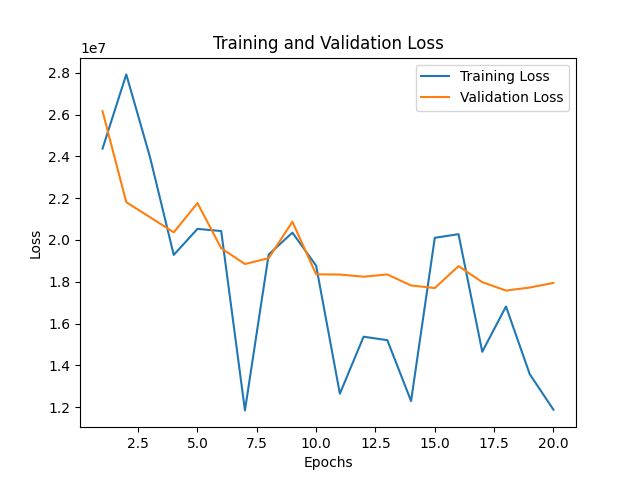
\includegraphics[width=\textwidth]{media/epochs.png}
    \label{fig:graphic1}
    \caption*{Fig. 1: Training and validation loss for different epochs}
  \end{subfigure}%
  \begin{subfigure}[b]{0.5\textwidth}
    \centering
    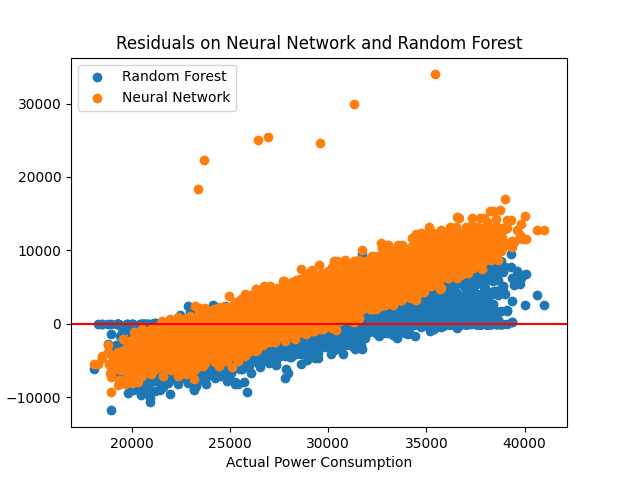
\includegraphics[width=\textwidth]{media/comparison_rf_nn.png}
    \label{fig:graphic2}
    \caption*{Fig. 2: Comparison neural network and random forest}
  \end{subfigure}
  \label{fig:graphics}
\end{figure*}


\section{Results}
\label{sec:results}
We checked the mean absolute error (MAE) for our three models. MAE is advantageous because it gives equal weight to all errors, regardless of their direction (positive or negative). It provides a simple and interpretable measure of how close the predictions are to the true values. A lower MAE indicates better predictive performance.
Our best model was the random forest, follow by the linear regression and neural network. Details of our results are discussed in \ref{sec:discuss}. In Figure 2 we compare the performance of the neural network and the random forest. 


\section{Discussion}
\label{sec:discuss}


Upon analyzing the data, we observed that both the linear regression model and the neural network displayed similar performance. Linear regression gives us a MAE of approximately 3100, the neural network around 3500. This implies that, in terms of prediction accuracy, these two models returned comparable results.

However, the random forest algorithm was the best in this particular scenario. Its MAE of approximately 1700 significantly outperformed both the linear regression model and the neural network. This indicates that the random forest algorithm, which uses multiple decision trees and combines their predictions, performed better in making accurate predictions compared to other methods in this particular situation.

During the development process, decision trees were initially explored, but they were quickly replaced with the random forest algorithm due to its benefits. Decision trees tend to overfit, have high variance and are sensitive to outliers. By replacing it with a random forest we got rid of these disadvantages. 

We tested different combinations of hyperparameters to see which ones made the model perform the best. We looked at things like the learning rate, the number of hidden layers, the number of neurons in each layer, and the activation functions used. We also tried different optimizers but they all resulted in about the same results. We also tried techniques to prevent the model from overfitting the data, like dropout and weight\_decay. The regularization techniques all lead to about the same result. 
We also trained our model with different amount of epochs, and after the tenth epoch the MAE converged. After trying different settings and comparing the results, we chose the best combination of hyperparameters.


It is likely that we did not optimize the pre-processing steps of the data enough.
An obvious way to try to improve our results could be more finetuning with the hyperparameters of the neural network and the random forest. 
We could also try other types of regression like multiple regression, ridge regression and k-nearest neighbors.
\section{Conclusion}
\label{sec:con}

When evaluating the performance of the linear regression and neural network models on the test set, we observed similar results to those obtained during the training phase. However, the random forest model showed a significant decline in estimation when tested on the test dataset compared to our validation dataset. The mean absolute error of the random forest increased from approximately 1700 on our validation set to 2200 on the test dataset.\\
The key lesson from this project was to explore different approaches and models using existing libraries instead of building everything from scratch. We also learned the importance of fine-tuning hyperparameters and observing their impact on the results.
Choosing the right prediction model for the problem was a challenging task. Surprisingly, the non-parametric approach using a random forest performed better than the other models. We expected the neural network to be the best performer.



%%%%%%%%%%%%%%%%%%%%%%%%%%%%%%%%%%%%%%%%%%%%%%%%%%%%%%%%%%%%%%%%%%%%%%%%%%%%%%%%



\end{document}
